\section{Mức độ 5,6 điểm}
\Opensolutionfile{ans}[ans/CD4/Muc_5_6]
\setcounter{dang}{0}
\setcounter{ex}{0}
\begin{dang}
	{Xác định đường tiệm cận thông qua bảng biến thiên, đồ thị}
\end{dang}
\begin{ex}[BGD-Minh Họa 1-2017]%[2D1Y4-4]
	Cho hàm số $y=f(x)$ có $\lim\limits_{x\rightarrow +\infty}y=1$ và $\lim\limits_{x\rightarrow -\infty}y=-1$. Khẳng định nào sau đây là khẳng định đúng?
	\choice
	{Đồ thị hàm số đã cho không có tiệm cận ngang}
	{Đồ thị hàm số đã cho có đúng một tiệm cận ngang}
	{\True Đồ thị hàm số đã cho có hai tiệm cận ngang là các đường thẳng $y=1$ và $y=-1$}
	{Đồ thị hàm số đã cho có hai tiệm cận ngang là các đường thẳng $x=1$ và $x=-1$}
	\loigiai{
		Theo định nghĩa đường tiệm cận, ta có:
		\begin{itemize}
			\item $\lim\limits_{x\rightarrow +\infty}y=1$ suy ra $ y=1 $ là đường tiệm cận ngang.
			\item $\lim\limits_{x\rightarrow -\infty}y=-1$ suy ra $ y=-1 $ là đường tiệm cận ngang.
		\end{itemize}
	}
\end{ex}

%%==========Câu 2
\begin{ex}[BGD-Minh Họa-2020-L2]%[2D1Y4-1]
	Tiệm cận ngang của đồ thị hàm số $y=\dfrac{x-2}{x+1}$ có phương trình là
	\choice
	{$y=-2$}
	{\True $y=1$}
	{$x=-1$}
	{$x=2$}
	\loigiai
	{
		Tập xác định: $\mathscr{D}=\mathbb{R}\setminus \{-1\}$.\\
		Ta có $\lim \limits_{x \to +\infty} y=\lim \limits_{x \to +\infty} \dfrac{x-2}{x+1}=\lim \limits_{x \to +\infty} \dfrac{1-\dfrac{2}{x}}{1+\dfrac{1}{x}}=1$ và $\lim \limits_{x \to -\infty} y=\lim \limits_{x \to -\infty} \dfrac{x-2}{x+1}=\lim \limits_{x \to -\infty} \dfrac{1-\dfrac{2}{x}}{1+\dfrac{1}{x}}=1$ nên đường thẳng $y=1$ là đường tiệm cận ngang của đồ thị.
	}
\end{ex}

%%==========Câu 3
\begin{ex}[BGD-THPT-2020-101-L1]%[2D1Y4-1]
	Tiệm cận ngang của đồ thị hàm số $y=\dfrac{4x+1}{x-1}$ có phương trình là
	\choice
	{$y=\dfrac{1}{4}$}
	{\True $y=4$}
	{$y=1$}
	{$y=-1$}
	\loigiai{
		Do $\lim\limits_{x\to \pm\infty} y = \lim\limits_{x\to \pm\infty}\dfrac{4x+1}{x-1}=4$ nên $y=4$ là tiệm cận ngang của đồ thị hàm số $y=\dfrac{4x+1}{x-1}$.
	}
\end{ex}

%%==========Câu 4
\begin{ex}[BGD-THPT-2020-102-L1]%[2D1B4-1]
	Tiệm cận ngang của đồ thị hàm số $y=\dfrac{5x+1}{x-1}$ có phương trình  là
	\choice
	{$y=1$}
	{$y=\dfrac{1}{5}$}
	{$y=-1$}
	{\True $y=5$}
	\loigiai{
		Ta có $ \lim\limits_{x\rightarrow \pm\infty}\dfrac{5x+1}{x-1}=\lim\limits_{x\rightarrow \pm\infty}\dfrac{5+\dfrac{1}{x}}{1-\dfrac{1}{x}}=5$.\\
		Vậy tiệm cận ngang của đồ thị hàm số đã cho là $y=5$.
	}
\end{ex}

%%==========Câu 5
\begin{ex}[BGD-THPT-2020-103-L1]%[2D1B4-1]
	Tiệm cận ngang của đồ thị hàm số $y=\dfrac{2x+1}{x-1}$ có phương trình là
	\choice
	{$y=\dfrac{1}{2}$}
	{$y=-1$}
	{$y=1$}
	{\True$y=2$}
	\loigiai{
		Ta có: $\lim\limits_{x\to \pm\infty}y=2$, nên tiệm cận ngang của đồ thị hàm số là $y = 2$.
	}
\end{ex}

%%==========Câu 6
\begin{ex}[BGD-THPT-2020-104-L1]%[2D1Y4-1]
	Tiệm cận ngang của đồ thị hàm số $y=\dfrac{3x+1}{x-1}$ có phương trình là
	\choice
	{$y=\dfrac{1}{3}$}
	{\True $y=3$}
	{$y=-1$}
	{$y=1$}
	\loigiai{
		Ta có $\lim\limits_{x\to\pm\infty}y=3$ nên $y=3$ là tiệm cận ngang của đồ thị hàm số đã cho.
	}
\end{ex}


%%==========Câu 7
\begin{ex}[BGD-THPT-2020-101-L2]%[2D1Y4-1]
	Tiệm cận đứng của đồ thị hàm số $y=\dfrac{2x+2}{x-1}$ có phương trình là
	\choice
	{$x=2$}
	{$x=-2$}
	{\True $x=1$}
	{$x=-1$}
	\loigiai{
		Tập xác định $\mathscr{D}=\mathbb{R}\setminus \{1\}$.\\
		Ta có $\lim\limits_{x\to 1^+}y=+\infty$, $\lim\limits_{x\to 1^-}y=-\infty$ nên đường thẳng $x=1$ là tiệm cận đứng của đồ thị hàm số $y=\dfrac{2x+2}{x-1}$.
	}
\end{ex}


%%==========Câu 8
\begin{ex}[BGD-THPT-2020-102-L2]%[2D1Y4-1]
	Tiệm cận đứng của đồ thị hàm số $y=\dfrac{x-1}{x-3}$ có phương trình là
	\choice
	{$x=-3$}
	{$x=-1$}
	{$x=1$}
	{\True $x=3$}
	\loigiai{
		Tập xác định $\mathscr D=\mathbb{R}\setminus \{3\}$.\\
		Ta có $\lim\limits_{x\to 3^{+}} y=+\infty$ và $\lim\limits_{x\to 3^{-}} y=-\infty$.\\
		Suy ra đồ thị hàm số đã cho có đường tiệm cận đứng là $x=3$.
	}
\end{ex}

%%==========Câu 9
\begin{ex}[BGD-THPT-2020-103-L2]%[2D1Y4-1]
	Tiệm cận đứng của đồ thị hàm số $y=\dfrac{2x-2}{x+1}$ có phương trình là 
	\choice
	{$x=-2$}
	{$x=1$}
	{\True $x=-1$}
	{$x=2$}
	\loigiai{Tiệm cận đứng của đồ thị hàm số $y=\dfrac{2x-2}{x+1}$ là $x=-1$.
	}
\end{ex}

%%==========Câu 10
\begin{ex}[BGD-THPT-2020-104-L2]%[2D1Y4-1]
	Tiệm cận đứng của đồ thị hàm số $y=\dfrac{x+1}{x+3}$ có phương trình là 
	\choice
	{$x=-1$}
	{$x=1$}
	{\True $x=-3$}
	{$x=3$}
	\loigiai{
		Tập xác định của hàm số đã cho $\mathscr{D}=\mathbb{R}\setminus\{-3\}$.\\
		Ta có $\lim\limits_{x\rightarrow-3^-}y=\lim\limits_{x\rightarrow-3^-}\dfrac{x+1}{x+3}=+\infty$ và $\lim\limits_{x\rightarrow-3^+}y=\lim\limits_{x\rightarrow-3^+}\dfrac{x+1}{x+3}=-\infty$.\\
		Khi đó đường tiệm cận đứng của đồ thị hàm số đã cho là $x=-3$.
	}
\end{ex}


%%==========Câu 11
\begin{ex}[BGD-Minh Họa-2020-L2]%[2D1Y4-1]
	Tiệm cận ngang của đồ thị hàm số $y=\dfrac{x-2}{x+1}$ có phương trình là
	\choice
	{$y=-2$}
	{\True $y=1$}
	{$x=-1$}
	{$x=2$}
	\loigiai
	{
		Tập xác định: $\mathscr{D}=\mathbb{R}\setminus \{-1\}$.\\
		Ta có $\lim \limits_{x \to +\infty} y=\lim \limits_{x \to +\infty} \dfrac{x-2}{x+1}=\lim \limits_{x \to +\infty} \dfrac{1-\dfrac{2}{x}}{1+\dfrac{1}{x}}=1$ và $\lim \limits_{x \to -\infty} y=\lim \limits_{x \to -\infty} \dfrac{x-2}{x+1}=\lim \limits_{x \to -\infty} \dfrac{1-\dfrac{2}{x}}{1+\dfrac{1}{x}}=1$ nên đường thẳng $y=1$ là đường tiệm cận ngang của đồ thị.
	}
\end{ex}


%%==========Câu 12
\begin{ex}[BGD-THPT-2021-101-L1]%[2D1Y4-1]
	Tiệm cận đứng của đồ thị hàm số $ y=\dfrac{2x-1}{x-1}$ là đường thẳng có phương trình là
	\choice
	{\True $x=1$}
	{$x=-1$}
	{$x=2$}
	{$x=\dfrac{1}{2}$}
	\loigiai{
		Vì $\lim\limits_{x\to 1^+}\dfrac{2x-1}{x-1}=+\infty $ và $\lim\limits_{x\to 1^-}\dfrac{2x-1}{x-1}=-\infty $ nên đồ thị hàm số $ y=\dfrac{2x-1}{x-1}$ có một tiệm cận đứng là đường thẳng $ x=1 $.
	}
\end{ex}

%%==========Câu 13
\begin{ex}[BGD-THPT-2021-102-L1]%[2D1Y4-1]
	Tiệm cận đứng của đồ thị hàm số $ y=\dfrac{x+1}{x-2}$ là đường thẳng có phương trình là
	\choice
	{$x=-1$}
	{$x=-2$}
	{\True $x=2$}
	{$x=1$}
	\loigiai{
		Ta có $\displaystyle\lim\limits_{x\to 2^+}\dfrac{x+1}{x-2}=+\infty $;  $\displaystyle\lim\limits_{x\to 2^-}\dfrac{x+1}{x-2}=-\infty $.\\
		Vậy đồ thị hàm số $ y=\dfrac{x+1}{x-2}$ có tiệm cận đứng là đường thẳng $ x=2 $.
	}
\end{ex}


%%==========Câu 14
\begin{ex}[BGD-THPT-2021-103-L1]%[2D1B4-1]
	Tiệm cận đứng của đồ thị hàm số $ y=\dfrac{2x+1}{x-1}$ là đường thẳng có phương trình là
	\choice
	{$x=2$}
	{\True $x=1$}
	{$x=-\dfrac{1}{2}$}
	{$x=-1$}
	\loigiai{
		Ta có $\lim\limits_{x\to 1^+}y=\lim\limits_{x\to 1^+}\dfrac{2x+1}{x-1}=+\infty $ nên tiệm cận đứng của đồ thị hàm số là đường thẳng $ x=1 $.
	}
\end{ex}

%%==========Câu 15
\begin{ex}[BGD-THPT-2021-104-L1]%[2D1Y4-1]
	Tiệm cận đứng của đồ thị hàm số $ y=\dfrac{x-1}{x+2}$ là đường thẳng có phương trình là
	\choice
	{$x=2$}
	{$x=-1$}
	{\True $x=-2$}
	{$x=1$}
	\loigiai{
		Ta có $\lim\limits_{x\to (-2)^{+}}\dfrac{x-1}{x+2}=-\infty $, $\lim\limits_{x\to (-2)^{-}}\dfrac{x-1}{x+2}=+\infty $.\\ 
		Đồ thị hàm số có tiệm cận đứng là đường thẳng có phương trình $ x=-2 $.
	}
\end{ex}


%%==========Câu 16
\begin{ex}[BGD-THPT-2019-103]%[2D1B4-1]
	Cho hàm số $y=f(x)$ có bảng biến thiên như sau
	\begin{center}
		
\begin{tikzpicture}[scale=1, font=\footnotesize,line join=round, >=stealth]
			\tkzTabInit[nocadre=false,lgt=1.5,espcl=3]{$x$/.7,$y'$/.7,$y$/2.5}{$-\infty$,$0$,$3$,$+\infty$}%
			\tkzTabLine{,-,d,+,0,-,}%
			\tkzTabVar{+/$1$ , -D+/$-\infty$/$2$,-/$-3$, +/$3$}%
		\end{tikzpicture}
	\end{center}
	Tổng số tiệm cận đứng và tiệm cận ngang của đồ thị hàm số đã cho là
	\choice
	{1}
	{2}
	{\True 3}
	{4}
	\loigiai{
		Nhìn bảng biến thiên ta thấy\\
		$\lim\limits_{x \to 0^-} f(x)=-\infty  \Rightarrow x=0$ là TCĐ của đồ thị hàm số.\\
		$\lim\limits_{x \to +\infty} f(x)=3 \Rightarrow y=3$ là TCN của đồ thị hàm số.\\
		$\lim\limits_{x \to -\infty} f(x)=1 \Rightarrow y=1$ là TCN của đồ thị hàm số.\\
		Vậy hàm số có 3 tiệm cận.}
\end{ex}


%%==========Câu 17
\begin{ex}[BGD-THPT-2019-102]%[2D1B4-1]
	Cho hàm số $f(x)$ có bảng biến thiên như sau
	\begin{center}
		
\begin{tikzpicture}[scale=1, font=\footnotesize,line join=round, >=stealth]
			\tkzTabInit[lgt=1.2,espcl=3]
			{$x$/0.8,$f’(x)$/0.8,$f(x)$/2}
			{$-\infty$,$0$,$1$,$+\infty$}
			\tkzTabLine{ ,-,d,-,0,+,}
			\tkzTabVar{+/$0$,-D+/$-\infty$/$2$,-/$-2$,+/$+\infty$}
		\end{tikzpicture}
	\end{center}
	Tổng số tiệm cận đứng và tiệm cận ngang của đồ thị hàm số đã cho là 
	\choice
	{$3$}
	{$1$}
	{\True $2$}
	{$4$}
	\loigiai{
		Từ bảng biến thiên đã cho ta có\\
		$\lim\limits_{x \to -\infty} f(x)=0$ nên đường thẳng $y=0$ là một tiệm cận ngang của đồ thị hàm số.\\
		$\lim\limits_{x \to 0^-} f(x)=-\infty$ nên đường thẳng $x=0$ là một tiệm cận đứng của đồ thị hàm số.\\
		Vậy đồ thị hàm số đã cho có hai đường tiệm cận.}
\end{ex}


%%==========Câu 18
\begin{ex}[BGD-THPT-2019-101]%[2D1B4-1]
	Cho hàm số $y=f(x)$ có bảng biến thiên như sau
	\begin{center}
		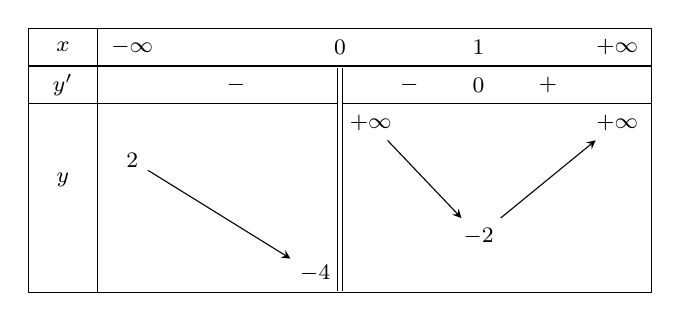
\begin{tikzpicture}[scale=0.8, font=\footnotesize, line join=round,>=stealth,yscale=.6,xscale=1.1]
			\def\cot{8} % số nhãn chiều dài
			\def\hang{6} % số nhãn chiều cao
			\draw[shift={(-.5,.5)}] 
			(0,0) rectangle +(\cot+1,-\hang-1)
			(0,-1)--+(0:\cot+1) 
			(0,-2)--+(0:\cot+1) 
			(1,0)--+(-90:\hang+1);		
			\path 
			(0,0) node{$x$} (1,0) node{$-\infty$}	(4,0) node{$0$} (6,0) node{$1$} (8,0)  node{$+\infty$}
			(0,-1) node{$y'$} (2.5,-1) node{$-$} (5,-1) node{$-$} (6,-1) node{$0$} (7,-1) node{$+$}	
			(0,-3.5) node{$y$}
			(1,-3) node (2) {$2$}							
			(4,-6) node[left] (-4) {$-4$}
			(4,-2) node[right] (khongR) {$+\infty$}
			(6,-5) node (CT) {$-2$}
			(8,-2) node (dvc) {$+\infty$};
			\draw[double, double distance=1.5pt] (4,-0.55)--(4,-6.45); %Không xác định
			\draw[->] (2)--(-4);		
			\draw[->] (khongR)--(CT);
			\draw[->] (CT)--(dvc);
		\end{tikzpicture}
	\end{center}
	Tổng số tiệm cận đứng và tiệm cận ngang của đồ thị hàm số đã cho là
	\choice
	{$4$}
	{$1$}
	{$3$}
	{\True $2$}
	\loigiai{
		Hàm số $y=f(x)$ có tập xác định $\mathscr{D}=\mathbb{R} \setminus \{0\}$.\\
		Ta có\\
		$\lim\limits_{x \to +\infty} f(x)=+\infty$ suy ra không tồn tại tiệm cận ngang khi $x \to +\infty$. \\
		$\lim\limits_{x \to -\infty} f(x)=2$, suy ra đồ thị hàm số $y=f(x)$ có tiệm cận ngang $y=2$.\\
		$\lim\limits_{x \to 0^+} f(x)=+\infty$; $\lim\limits_{x \to 0^-} f(x)=-4$, suy ra đồ thị hàm số $y=f(x)$ có tiệm cận đứng $x=0$. \\
		Vậy tổng số tiệm cận đứng và ngang là $2$.}
\end{ex}

%%==========Câu 19
\begin{ex}[BGD-Minh Họa-2019]%[2D1B4-1]
	
	\immini{Cho hàm số $y=f(x)$ có bảng biến thiên như hình bên. Tổng số tiệm cận ngang và tiệm cận đứng của đồ thị hàm số đã cho là
		\choice
		{$4$.\hspace{.25\linewidth}}
		{$1$}
		{\True $3$}
		{$2$}
	}
	{
\begin{tikzpicture}[scale=0.8, font=\footnotesize,line join=round, >=stealth]
			\tikzset{double style/.append style ={draw=\tkzTabDefaultWritingColor,double=\tkzTabDefaultBackgroundColor,double distance=2pt}}
			\tikzset{h style/.style ={pattern=north west lines}}
			\tkzTabInit[nocadre=false,lgt=1.5,espcl=3.5]
			{$x$/.7,$ $/0,$f(x)$ /2}
			{$-\infty$,$1$,$+\infty$}
			\tkzTabLine{ , ,d, , }
			\tkzTabVar{-/$2$,+D-/$+\infty$/$3$,+/$5$ }
	\end{tikzpicture}}
	
	\loigiai{
		Dựa vào bảng biến thiên, suy ra:\\
		$\displaystyle \lim_{x\to-\infty}y=2\Rightarrow y=2$ là tiệm cận ngang.\\
		$\displaystyle \lim_{x\to+\infty}y=5\Rightarrow y=5$ là tiệm cận ngang.\\
		$\displaystyle \lim_{x\to1^+}y=+\infty\Rightarrow x=1$ là tiệm cận đứng.\\
		Vậy tổng số tiệm cận ngang và tiệm cận đứng là $3$.
	}
\end{ex}


%%==========Câu 20
\begin{ex}[THPT Yên Định - Thanh Hóa 2019]%[2D1B4-1]
	Cho hàm số $ y=f(x) $ xác định và có đạo hàm trên $ \mathbb{R}\setminus\{\pm 1\} $. Hàm số có bảng biến thiên như hình vẽ dưới đây.
	\begin{center}
		
\begin{tikzpicture}[scale=1, font=\footnotesize,line join=round, >=stealth]
			\tkzTabInit[nocadre=false,lgt=1.2,espcl=2.5,deltacl=0.6]{$x$/.6 ,$y'$/.6,$y$/2.5} {$-\infty$ , $-1$ , $0$ , $1$ , $+\infty$}
			\tkzTabLine{ , + , d , - , d , + ,  d , + , }
			\tkzTabVar{-/$-4$ , +D-/$+\infty$/$-\infty$ , +/$2$,-D-/$-\infty$/$-\infty$,+/$-1$}
		\end{tikzpicture}
	\end{center}
	Tổng số đường tiệm cận đứng và tiệm cận ngang của đồ thị hàm số đã cho là
	\choice
	{ $ 1 $ }
	{ $ 2 $ }
	{ $ 3 $ }
	{\True  $ 4 $ }
	\loigiai{
		Dựa vào bảng biến thiên, suy ra:\\
		$ \lim \limits_{x \to - \infty} y=-4 $, $ \lim \limits_{x \to + \infty} y=-1$. Đồ thị có hai tiệm cận ngang là $ y=-4 $ và $ y=-1 $.\\
		Lại có $  \lim \limits_{x \to (-1)^+} y=+\infty  $ và $ \lim \limits_{x \to  1^-} y=+\infty $, $ \lim \limits_{x \to 1^-} y=-\infty $. Đồ thị hàm số có hai đường tiệm cận đứng là $ x=1 $ và $ x=-1 $.
	}
\end{ex}
\begin{ex}%[2D1B4-1]
	(Đề tham khảo 2017) Cho hàm số $y=f\left(x\right)$ có bảng biến thiên như hình vẽ dưới đây. 
	\begin{center}\vspace*{-1cm}
		\begin{tikzpicture}[line cap=round,line join=round,>=triangle 45,x=1.0cm,y=1.0cm]
			\clip(-1.58,-2.4) rectangle (12.58,2.);
			\fill[line width=1.2pt,dash pattern=on 15 pt off 5pt,color=white,fill=black,pattern=north east lines,pattern color=black] (0.,1.) -- (2.84,1.) -- (2.84,-1.96) -- (0.,-1.96) -- cycle;
			\draw (-1.,1.)-- (12.,1.);
			\draw (-1.,0.)-- (12.,0.);
			\draw (0.,1.62)-- (0.,-1.96);
			\draw (0.08,1.5) node[anchor=north west] {$-\infty$};
			\draw (2.46,1.5) node[anchor=north west] {$-2$};
			\draw (6.85,1.5) node[anchor=north west] {$0$};
			\draw (11.14,1.5) node[anchor=north west] {$+\infty$};
			\draw (2.84,1.)-- (2.84,-1.96);
			\draw (3.,1.)-- (3.,-1.96);
			\draw (7.,1.)-- (7.,-1.96);
			\draw (7.14,1.)-- (7.14,-1.96);
			\draw (-0.7,1.5) node[anchor=north west] {$x$};
			\draw (-0.72,0.78) node[anchor=north west] {$y'$};
			\draw (-0.64,-0.8) node[anchor=north west] {$y$};
			\draw [->] (3.96,-1.54) -- (6.24,-0.64);
			\draw [->] (7.64,-0.58) -- (11.12,-1.7);
			\draw (11.34,-1.5) node[anchor=north west] {$0$};
			\draw (8.98,0.7) node[anchor=north west] {$-$};
			\draw (4.68,0.7) node[anchor=north west] {$+$};
			\draw (6.0,-0.2) node[anchor=north west] {$+\infty$};
			\draw (7.22,-0.2) node[anchor=north west] {$1$};
			\draw (3.08,-1.5) node[anchor=north west] {$-\infty$};
		\end{tikzpicture}
	\end{center}
	Hỏi đồ thị của hàm số đã cho có bao nhiêu đường tiệm cận? 
	\choice
	{\True $3$}
	{$2$}
	{$4$}
	{$1$}
	\loigiai{
		Dựa vào bảng biến thiên ta có:\\
		$\lim\limits_{x \to -2^{+}} f(x)=-\infty$, suy ra đường thẳng $x=-2$ là tiệm cận đứng của đồ thị hàm số.\\
		$\lim\limits_{x \to  0^{-}} f(x)=+\infty$, suy ra đường thẳng $x=0$ là tiệm cận đứng của đồ thị hàm số.\\
		$\lim\limits_{x \to +\infty} f(x)=0$, suy ra đường thẳng $y=0$ là tiệm cận ngang của đồ thị hàm số.\\
		Vậy đồ thị hàm số có $3$ đường tiệm cận.}
\end{ex}

\begin{ex}%[2D1B4-1]
	(Mã 104 - 2019) Cho hàm số $y=f\left(x\right)$ có bảng biến thiên như sau:
	\begin{center}
		
\begin{tikzpicture}[scale=1,line join=round,>=stealth]\tikzset{double style/.append style={double distance=2pt}}
			\tkzTabInit[nocadre=false,lgt=1.2,espcl=2.5,deltacl=0.6]
			{$x$ /0.6,$y'$ /0.6,$y$ /2}
			{$ -\infty $,$0$,$3$,$+\infty$}
			\tkzTabLine{,-,d,-,0,+}
			\tkzTabVar{+/$0$,-D+/$-4$/$+\infty$,-/$-3$,+/$3$,}
		\end{tikzpicture}
	\end{center}
	Tổng số tiệm cận đứng và tiệm cận ngang của đồ thị hàm số đã cho là
	\choice
	{$1$}
	{\True $3$}
	{$4$}
	{$2$}
	\loigiai{
		Ta có $\lim\limits_{x \to +\infty} f(x)=3$ và $\lim\limits_{x \to -\infty} f(x)=0$ nên đồ thị hàm số có $2$ tiệm cận ngang là các đường thẳng có phương trình $y=3$ và $y=0$.\\
		Lại có $\lim\limits_{x \to  0^{+}} f(x)=+\infty$ nên hàm số có $1$ tiệm cận đứng là đường thẳng có phương trình $x=0$.}
\end{ex}

\begin{ex}%[2D1B4-1]
	(Chuyên Lê Quý Đôn Điện Biên 2019) Cho hàm số $f(x)$ có bảng biến thiên như sau:
	\begin{center}
		
\begin{tikzpicture}[scale=1,line join=round,>=stealth]\tikzset{double style/.append style={double distance=2pt}}
			\tkzTabInit[nocadre=false,lgt=1.2,espcl=2.5,deltacl=0.6]
			{$x$ /0.6,$f(x)$ /2.5}
			{$ -\infty $,$-2$,$+\infty$}
			\tkzTabVar{-/$-\infty$,+D-/$+\infty$/$1$,+/$3$, }
		\end{tikzpicture}
	\end{center}
	Tổng số tiệm cận ngang và tiệm cận đứng của đồ thị hàm số đã cho là
	\choice
	{$4$}
	{$3$}
	{$1$}
	{\True $2$}
	\loigiai{Dựa vào bảng biến thiên ta có:\\
		$\lim\limits_{x \to +\infty} f(x)=3$ ta được tiệm cận ngang $y=3$.\\
		$\lim\limits_{x \to (-2)^{-}} f(x)=+\infty$ ta được tiệm cận đứng $x=-2$.}
\end{ex}

\begin{ex}%[2D1B4-1]
	(Liên Trường THPT TP Vinh Nghệ An 2019) Cho hàm số $y=f\left(x\right)$ có bảng biến thiên như sau:
	\begin{center}
		
\begin{tikzpicture}[scale=1,line join=round,>=stealth]\tikzset{double style/.append style={double distance=2pt}}
			\tkzTabInit[nocadre=false,lgt=1.2,espcl=2.5,deltacl=0.6]
			{$x$ /0.6,$y$ /2.5}
			{$ -\infty $,$-2$,$+\infty$}
			\tkzTabVar{+/$-5$,-D+/$-\infty$/$1$,-/$-5$, }
		\end{tikzpicture}
	\end{center}
	Tổng số tiệm cận ngang và tiệm cận đứng của đồ thị hàm số đã cho là
	\choice
	{$4$}
	{\True $2$}
	{$3$}
	{$1$}
	\loigiai{
		Từ bảng biến thiên ta có:
		\begin{itemize}
			\item $\lim\limits_{x \to \pm\infty} y=-5$ nên tiệm cận ngang là $y=-5$.
			\item $\lim\limits_{x \to -2^-} y=-\infty$ nên tiệm cận đứng là $x=2$.
		\end{itemize}
		Vậy đồ thị hàm số đã cho có $2$ tiệm cận.
	}
\end{ex}

\begin{ex}%[2D1B4-1]
	(THPT Hùng Vương Bình Phước 2019) Cho đồ thị hàm số $y=f\left(x\right)$ như hình bên dưới. 
	\begin{center}
		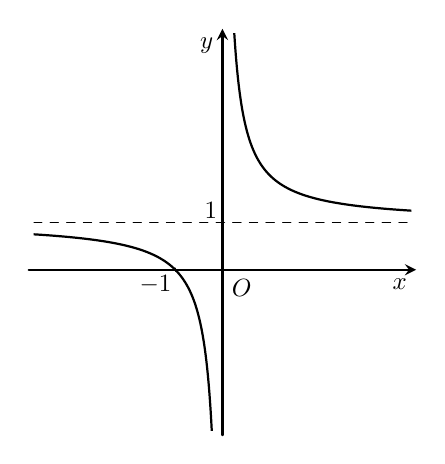
\begin{tikzpicture}[line join=round, line cap=round,>=stealth,thick,scale=0.6]
			\tikzset{every node/.style={scale=0.9}}
			\draw[->] (-4.1,0)--(4.1,0) node[below left] {$x$};
			\draw[->] (0,-3.5)--(0,5.1) node[below left] {$y$};
			\draw (0,0) node [below right] {$O$};
			\foreach \x in {-1}
			\draw[thin] (\x,1pt)--(\x,-1pt) node [below left=-2pt] {$\x$};
			\foreach \y in {1}
			\draw[thin] (1pt,\y)--(-1pt,\y) node [above left=-2pt] {$\y$};
			%\draw[dashed,thin] (0.01,-3)--(0.01,3);
			\begin{scope}
				\clip (-4,-3.4) rectangle (4,5);
				\draw[samples=200,domain=-4:-0.01,smooth,variable=\x] plot (\x,{(1*(\x)+1)/(1*(\x)+0)});
				\draw[samples=200,domain=0.01:4,smooth,variable=\x] plot (\x,{(1*(\x)+1)/(1*(\x)+0)});
				\draw[dashed,thin] (-4,1/1)--(4,1/1);
			\end{scope}
		\end{tikzpicture}
	\end{center}
	Khẳng định nào sau đây là đúng?
	\choice
	{\True Đồ thị hàm số có tiệm cận đứng $x=0$, tiệm cận ngang $y=1$}
	{Hàm số có hai cực trị}
	{Đồ thị hàm số chỉ có một đường tiệm cận}
	{Hàm số đồng biến trong khoảng $(-\infty ; 0)$ và $(0 ;+\infty)$}
	\loigiai{
		Dựa vào đồ thị, ta có một tiệm cận ngang là $y=1$ và một tiệm cận đứng là $x=0$.
	}
\end{ex}

\begin{ex}%[2D1B4-1]
	Cho hàm số $f(x)$ có bảng biến thiên như sau:
	\begin{center}
		
\begin{tikzpicture}[scale=1,line join=round,>=stealth]\tikzset{double style/.append style={double distance=2pt}}
			\tkzTabInit[nocadre=false,lgt=1.2,espcl=2.5,deltacl=0.6]
			{$x$ /0.6,$y'$ /0.6,$y$ /2}
			{$ -\infty $,$0$,$1$,$+\infty$}
			\tkzTabLine{,+,0,-,d,+}
			\tkzTabVar{-/$0$,+/$2$,-D-/$-\infty$/$3$,+/$5$,}
		\end{tikzpicture}
	\end{center}
	Tổng số tiệm cận ngang và tiệm cận đứng của đồ thị hàm số đã cho là
	\choice
	{$4$}
	{$1$}
	{\True $3$}
	{$2$}
	\loigiai{
		Dựa vào bảng biến thiên của hàm số ta có:
		\begin{itemize}
			\item $\lim\limits_{x \to -\infty} f(x)=0 \Rightarrow y=0$ là một tiệm cận ngang.
			\item $\lim\limits_{x \to +\infty} f(x)=5 \Rightarrow y=5$ là một tiệm cận ngang.
			\item $\lim\limits_{x \to  1^{-}} f(x)=-\infty \Rightarrow x=1$ là một tiệm cận đứng.
		\end{itemize}
		Vậy đồ thị hàm số có tổng số đường tiệm cận là $3$.}
\end{ex}

\begin{ex}%[2D1B4-1]
	Cho hàm số $y=f\left(x\right)$ có bảng biến thiên như sau:
	\begin{center}
		
\begin{tikzpicture}[scale=1,line join=round,>=stealth]\tikzset{double style/.append style={double distance=2pt}}
			\tkzTabInit[nocadre=false,lgt=1.2,espcl=2.5,deltacl=0.6]
			{$x$/0.6,$y$/2.5}
			{$ -\infty $,$1$,$+\infty$}
			\tkzTabVar{-/$2$,+D-/$+\infty$/$-\infty$,+/$2$, }
		\end{tikzpicture}
	\end{center}
	Tổng số tiệm cận ngang và tiệm cận đứng của đồ thị hàm số đã cho là
	\choice
	{$4$}
	{$1$}
	{$3$}
	{\True $2$}
	\loigiai{
		Dựa vào bảng biến thiên của hàm số ta có
		\begin{itemize}
			\item $\lim\limits_{x \to  \pm \infty} f(x)=2 \Rightarrow y=2$ là  tiệm cận ngang.
			\item $\lim\limits_{x \to  1^{+}} f(x)=-\infty \Rightarrow x=1$ là  tiệm cận đứng.
		\end{itemize}
		Vậy đồ thị hàm số có tổng số đường tiệm cận là $2$.}
\end{ex}

\begin{ex}%[2D1B4-1]
	(Sở Hà Nội 2019) Cho hàm số $y=f\left(x\right)$ có bảng biến thiên như sau
	\begin{center}
		
\begin{tikzpicture}[scale=1,line join=round,>=stealth]\tikzset{double style/.append style={double distance=2pt}}
			\tkzTabInit[nocadre=false,lgt=1.2,espcl=2.2,deltacl=0.6]
			{$x$ /.6,$y'$ /.6,$y$ /2.2}
			{$ -\infty $,$-2$,$0$,$+\infty$}
			\tkzTabLine{,-,d,+,d,-}
			\tkzTabVar{+/$+\infty$,-D-/$1$/$-\infty$,+D+/$+\infty$/$1$,-/$0$,}
		\end{tikzpicture}
	\end{center}
	Tổng số đường tiệm cận đứng và tiệm cận ngang của đồ thị hàm số đã cho bằng
	\choice
	{$2$}
	{$1$}
	{$0$}
	{\True $3$}
	\loigiai{
		Ta có
		\begin{itemize}
			\item $\lim\limits_{x \to -2^{+}} y=-\infty \Rightarrow x=-2$ là tiệm cận đứng.
			\item $\lim\limits_{x \to  0^{-}} y=+\infty \Rightarrow x=0$ là tiệm cận đứng.
			\item $\lim\limits_{x \to +\infty} y=0 \Rightarrow y=0$ là tiệm cận ngang.
		\end{itemize}
		Vậy đồ thị hàm số đã cho có tổng đường tiệm cận đứng và tiệm cận ngang là $3$.}
\end{ex}

\begin{ex}%[2D1B4-1]
	Cho hàm số $y=f\left(x\right)$ liên tục trên $\mathbb{R} \backslash\{1\}$ có bảng biến thiên như bảng sau:  
	\begin{center}
		
\begin{tikzpicture}[scale=1,line join=round,>=stealth]
			\tikzset{double style/.append style={double distance=2pt}}
			\tkzTabInit[nocadre=false,lgt=1.2,espcl=2.8,deltacl=0.6]
			{$x$ /0.6,$y'$ /0.6,$y$ /2.2}
			{$ -\infty $,$-1$,$1$,$+\infty$}
			\tkzTabLine{,-,0,+,d,+}
			\tkzTabVar{+/$1$,-/$-\sqrt 2$,+D-/$+\infty$/$-\infty$,+/$-1$,}
		\end{tikzpicture}
	\end{center}
	Tổng số đường tiệm cận đứng và đường tiệm cận ngang của đồ thị hàm số $y=f\left(x\right)$ là
	\choice
	{$1$}
	{$4$}
	{$2$}
	{\True $3$}
	\loigiai{
		Do $\lim\limits_{x \to  1^{+}} y=-\infty \Rightarrow$ Tiệm cận đứng  $x=1$.\\
		Lại có $\lim\limits_{x \to +\infty} y=-1 ; \lim\limits_{x \to -\infty} y=1 \Rightarrow$ Đồ thị có $2$ tiệm cận ngang là $y=\pm 1$.\\
		Vậy, đồ thị hàm số đã cho có tổng số tiệm cận là $3$.}
\end{ex}

\begin{ex}%[2D1B4-1]
	(Cụm liên trường Hải Phòng 2019) Cho hàm số $y=f\left(x\right)$ có bảng biến như sau:
	\begin{center}
		
\begin{tikzpicture}[scale=1,line join=round,>=stealth]
			\tikzset{double style/.append style={double distance=2pt}}
			\tkzTabInit[nocadre=false,lgt=1.2,espcl=2.5,deltacl=0.6]{$x$ /.6,$y'$ /.6,$y$ /2}
			{$ -\infty $,$-3$,$3$,$+\infty$}
			\tkzTabLine{,+,d,+,d,+}
			\tkzTabVar{-/$0$,+D-/$+\infty$/$-\infty$,+D-/$+\infty$/$-\infty$,+/$0$,}
		\end{tikzpicture}
	\end{center}
	Số đường tiệm cận của đồ thị hàm số là
	\choice
	{\True $3$}
	{$1$}
	{$4$}
	{$2$}
	\loigiai{
		Từ bảng biến thiên của hàm số ta có
		\begin{itemize}
			\item $\lim\limits_{x \to -\infty} y=0 ; \lim\limits_{x \to +\infty} y=0 \Rightarrow$ Đường thẳng $y=0$ là tiệm cận ngang.
			\item $\lim\limits_{x \to (-3)^{-}} y=+\infty \Rightarrow$ Đường thẳng $x=-3$ là tiệm cận đứng.
			\item $+\lim\limits_{x \to  3^{-}} y=+\infty  \Rightarrow$ Đường thẳng $x=3$ là tiệm cận đứng.
		\end{itemize}
		Vậy số đường tiệm cận của đồ thị hàm số là $3$.}
\end{ex}

\begin{ex}%[2D1B4-1]
	(Thi thử cụm Vũng Tàu 2019) Cho hàm số $y=f\left(x\right)$ có bảng biến thiên như sau
	\begin{center}
		
\begin{tikzpicture}[scale=1,line join=round,>=stealth]
			\tikzset{double style/.append style={double distance=2pt}}
			\tkzTabInit[nocadre=false,lgt=1.2,espcl=2.5,deltacl=0.6]
			{$x$ /.6,$y'$ /.6,$y$ /2.2}
			{$ -\infty $,$-2$,$2$,$+\infty$}
			\tkzTabLine{,-,d,-,d,-}
			\tkzTabVar{+/$0$,-D+/$-\infty$/$+\infty$,-D+/$-\infty$/$+\infty$,-/$-\infty$,}
		\end{tikzpicture}
	\end{center}
	Tổng số tiệm cận đứng và tiệm cận ngang của đồ thị hàm số đã cho là
	\choice
	{$4$}
	{$2$}
	{\True $3$}
	{$1$}
	\loigiai{
		Dựa vào bảng biến thiên, ta có:
		\begin{itemize}
			\item $\lim\limits_{x \to -\infty} f(x)=0$ nên đường thẳng $y=0$ là đường tiệm cận ngang.
			\item $\lim\limits_{x \to -2^{+}} f(x)=+\infty $ nên đường thẳng $x=-2$ là đường tiệm cận đứng.
			\item $\lim\limits_{x \to  2^{+}} f(x)=+\infty$ nên đường thẳng $x=2$ là đường tiệm cận đứng.
		\end{itemize}
		Vậy, tổng số tiệm cận đứng và tiệm cận ngang của đồ thị hàm số đã cho là $3$.}
\end{ex}

\begin{ex}%[2D1B4-1]
	(Đề minh họa 2022) Tiệm cận đứng của đồ thị hàm số $y=\dfrac{3 x+2}{x-2}$ là đường thẳng có phương trình là
	\choice
	{\True $x=2$}
	{$x=-1$}
	{$x=3$}
	{$x=-2$}
	\loigiai{
		Ta có $\lim\limits_{x \to  2^{+}} y=\lim\limits_{x \to  2^{+}} \dfrac{3 x+2}{x-2}=+\infty, \lim\limits_{x \to  2^{-}} y=\lim\limits_{x \to  2^{-}} \dfrac{3 x+2}{x-2}=-\infty$. \\
		Vậy $x=2$ là tiệm cận đứng.}
\end{ex}

\begin{ex}%[2D1Y4-1]
	(Mã 101 - 2022) Tiệm cận ngang của đồ thì hàm số $y=\dfrac{2 x-1}{2 x+4}$ là đường thẳng có phương trình là
	\choice
	{$x=-2$}
	{$x=1$}
	{\True $y=1$}
	{$y=-2$}
	\loigiai{
		Ta có $\lim\limits_{x \to  \pm \infty} \dfrac{2 x-1}{2 x+4}=1$.\\ Vậy tiệm cận ngang của đồ là đường thẳng $y=1$.}
\end{ex}

\begin{ex}%[2D1Y4-1]
	(Mã 102 - 2022) Tiệm cận ngang của đồ thị hàm số $y=\dfrac{2 x-1}{2 x+4}$ là đường thẳng có phương trình là
	\choice
	{$y=-2$}
	{$x=-2$}
	{$x=1$}
	{\True $y=1$}
	\loigiai{
		Ta có $\lim\limits_{x \to +\infty} y=\lim\limits_{x \to +\infty} \dfrac{2 x-1}{2 x+4}=1$ và $\lim\limits_{x \to -\infty} y=\lim\limits_{x \to -\infty} \dfrac{2 x-1}{2 x+4}=1$.\\
		Vậy đồ thị hàm số có tiệm cận ngang là $y=1$.}
\end{ex}

%%Câu 35-36
\begin{ex}%[2D1Y4-1]
	(Mã 103 - 2022) Cho hàm số $ y=f(x) $ có bảng biến thiên như sau:
	\begin{center}
		
\begin{tikzpicture}[scale=1]
			\tikzset{double style/.append style={double distance=2pt}}
			\tkzTabInit[nocadre=false,lgt=1.2,espcl=2.5,deltacl=0.6]
			{$x$ /0.6,$y’$ /0.6,$y$ /2}
			{$-\infty$,$-2$,$+\infty$}
			\tkzTabLine{,-,d,-,}
			\tkzTabVar{+/$-1$,-D+/$-\infty$/$+\infty$,-/$-1$}
		\end{tikzpicture}
	\end{center}
	Tiệm cận đứng của đồ thị hàm số đã cho là đường thẳng có phương trình là
	\choice
	{$ x=-1 $}
	{$ y=-1 $}
	{$ y=-2 $}
	{\True $ x=-2 $}
	\loigiai
	{
		Ta có $ \lim \limits_{x \to -2^{+}} f(x) =+\infty$ và $ \lim \limits_{x \to -2^{-}} f(x) =-\infty$.\\Vậy đồ thị hàm số có tiệm cận đứng $ x=-2 $.
	}
\end{ex}
\begin{ex}%[2D1Y4-1]
	[Mã 104 - 2022] Cho hàm số $ y=f(x) $ có bảng biến thiên như sau:
	\begin{center}
		
\begin{tikzpicture}[scale=1]
			\tikzset{double style/.append style={double distance=1.5pt}}
			\tkzTabInit[nocadre=false,lgt=1.2,espcl=2.5,deltacl=0.6]
			{$x$ /0.6,$y’$ /0.6,$y$ /2}
			{$-\infty$,$-2$,$+\infty$}
			\tkzTabLine{,-,d,-,}
			\tkzTabVar{+/$-1$,-D+/$-\infty$/$+\infty$,-/$-1$}
		\end{tikzpicture}
	\end{center}
	Tiệm cận ngang của đồ thị hàm số đã cho là đường thẳng  có phương trình là
	\choice
	{\True $ y=-1 $}
	{$ y=-2 $}
	{$ x=-2 $}
	{$ x=-1 $}
	\loigiai
	{Ta có $ \lim \limits_{x \to \pm \infty} f(x) =-1$.\\Vậy đồ thị hàm số có tiệm cận ngang là đường thẳng $ y=-1 $.
	}
\end{ex}
\Closesolutionfile{ans}
\indapan{10}{ans/CD4/Muc_5_6}